
\documentclass[preprint,12pt]{elsarticle}

\usepackage[spanish]{babel}
\usepackage{amssymb}
\usepackage{graphicx}
\usepackage{lineno}
\usepackage[utf8]{inputenc}
\usepackage{url}
\usepackage{natbib}

\begin{document}
	
	\begin{frontmatter}

		\title{\huge PRACTICA DE LABORATORIO N° 04: Elaboración de Dashboards en Power BI	 }
		\author{	Tarqui Montalico,Risther(2017057469)}
		
		





\end{frontmatter}

%%INICIO Resumen
\section{Objetivo}
	
	Realizar con exito los pasos de la guia con PowerBI
%%FIN Resumen

\section{Desarrolo}

	
		\begin{itemize}
			
			\\ \item Paso 1: Para esta guía utilizaremos el cubo creado en la guía anterior. Inicie Power BI Desktop, busque y seleccione la opción Get Data
			
			
		
			\\ \itemPaso 2: Dentro de los resources seleccionaremos SQL Server database
			
				\\ 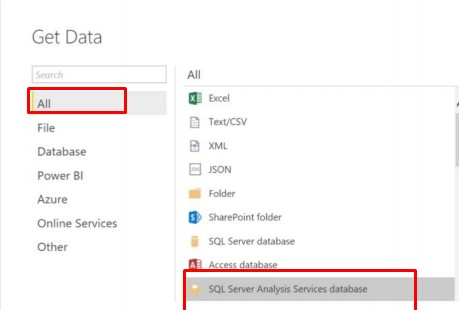
\includegraphics[width=7cm]{./IMAGENES/2} \\
			
			
			\\ \item Paso 3: Utilice el nombre de host o localhost para conectarse
			
			
				\\ 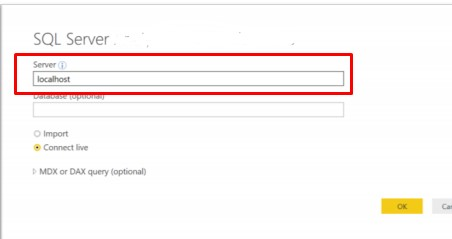
\includegraphics[width=7cm]{./IMAGENES/3} \\
			
			
			\\ \item Paso 4: Una vez conectado tendremos en nuestro lado dos toolbox, uno denominado VISUALIZATONS y otro denominado FIELDS.
			En FIELDS debe mostrar la Fact Table de Internet Sales y las dimensiones asociadas segdn las guias previas de cubos.
			
				\\ 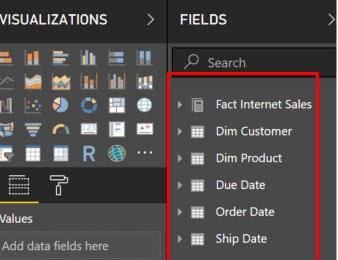
\includegraphics[width=7cm]{./IMAGENES/4} \\
			
			
			
			
			\\ \item  Paso 5: Vamos a crear nuestro primer reporte. Seleccionaremos una grâfica de barras, en segundo lugar Sales Amount, Calendar Year y English Product Name. (Debe hacerlo en ese orden).
			
				\\ 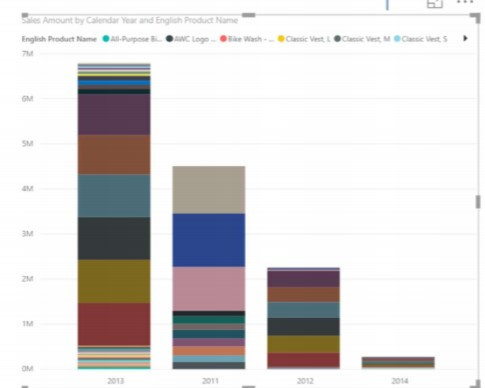
\includegraphics[width=7cm]{./IMAGENES/6} \\
			
			
			
			La grâfica resultante es la siguiente:
			
			
			
			
			
			
			\\ \item Paso 7: Elimine la grâfica anterior y procederâ a seleccionar grâfica de barras, en segundo lugar Sales Amount, English Product Name y Calendar Year. (Debe hacerlo en ese orden).
			
				\\ 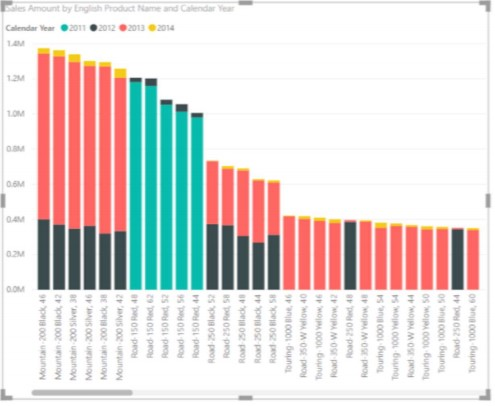
\includegraphics[width=7cm]{./IMAGENES/7} \\
			
			
			
			La grâfica cambiarâ, Io que indica que el orden de agregado es importante para las visualizaciones, adn habiendo seleccionado los mismos datos.
			
			
			\\ \item Paso 8: Cree un nuevo reporte.
			Podemos crear un dashboard con grâficos simultâneos. Arrastre dos grâficas y seleccione una de ella para establecer las propiedades.
			
				\\ 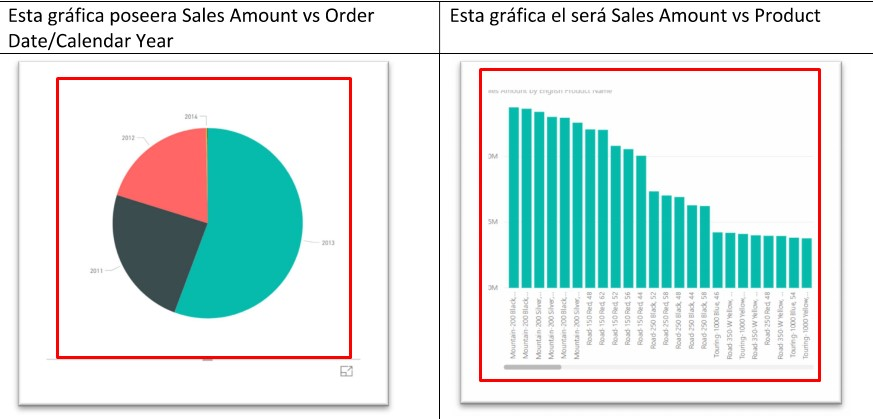
\includegraphics[width=7cm]{./IMAGENES/8} \\
			
			
			Esta grâfica poseera Sales Amount vs Order
			Date/Calendar Year	Esta grâfica el serâ Sales Amount vs Product
			
			
			
			
		\\ \item	Paso 10: Seleccione una de los valores de la grâfica de la izquierda para ver el comportamiento:
			
				\\ \includegraphics[width=7cm]{./IMAGENES/9} \\
			
			
			
			\\ \item Paso 11: Ahora crearemos un mapa que muestre la proporcién de ventas por zona geogrâfica. Arrastre un Mapa y una tabla
			
			
				\\ 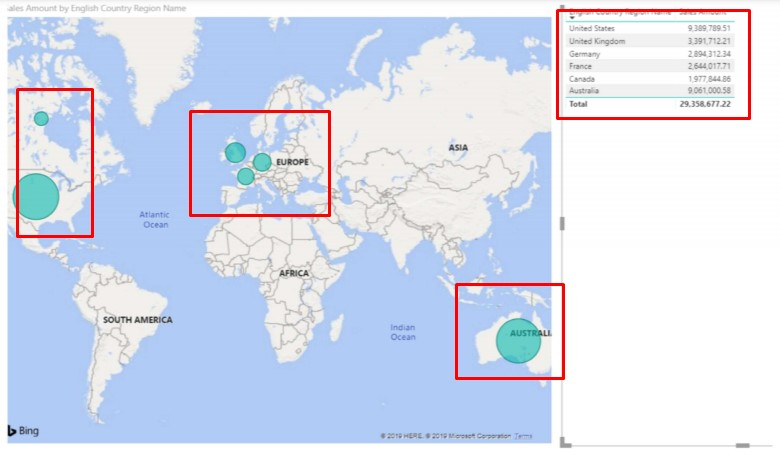
\includegraphics[width=7cm]{./IMAGENES/11} \\
			
			
		\\ \item	Paso 12: Ahora generaremos una grâfica de area.
			En primer lugar seleccione una nueva pagina y agregue una grâfica de area. Luego seleccione las medidas que se van a mostrar en el grâfico:
			
			
				\\ 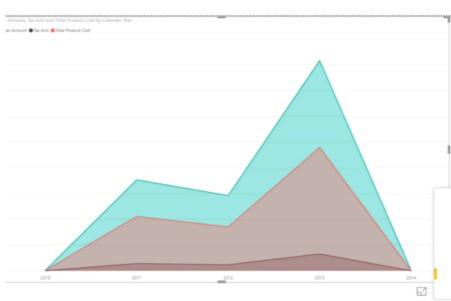
\includegraphics[width=7cm]{./IMAGENES/12} \\
		\\ \item	Paso 13: Agregaremos una grâfica de Ii'neas. Vamos a seleccionar desde la tabla de hecho a Sales Amount.
			A continuacion agregaremos Calendar Year desde Order Date y luego English Country Region Name. Debe realizarse en este orden o el resultado serâ diferente.
			
			
				\\ 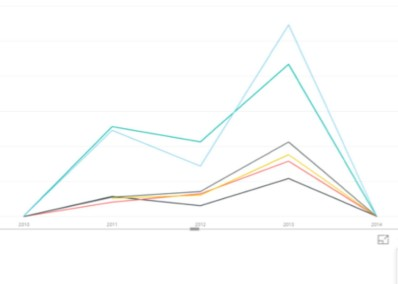
\includegraphics[width=7cm]{./IMAGENES/13} \\
			
			
			\\ \itemPaso 14: Puede definir los nombres de las hojas para indicar el tipo de reporte y la informacién. Establezca nombres descriptivos segdn la informacién que usted quiere facilitar.
			
			
				\\ 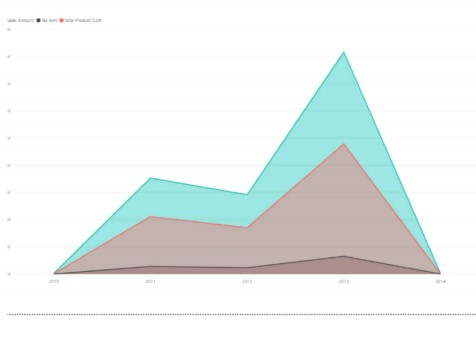
\includegraphics[width=7cm]{./IMAGENES/14} \\
			
			\\ \itemPaso 15: Crearemos un reporte (grâfico de barras) con filtrado bâsico. Seleccionar Sales Amount, English Country Region Name y Order date/Calendar Year. Buscarâ la seccién Basic Filtering y marcarâ Canada / United Kingdom.
			
			
			
				\\ 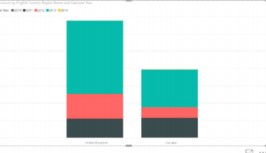
\includegraphics[width=7cm]{./IMAGENES/15} \\
			
			\\ \itemPaso 16: La siguiente grâfica es una Stacked Column Chart. Los atributos que utilizaremos son Sales Amount vs English ProductName vs Order Date/Calendar Year
			
				\\ 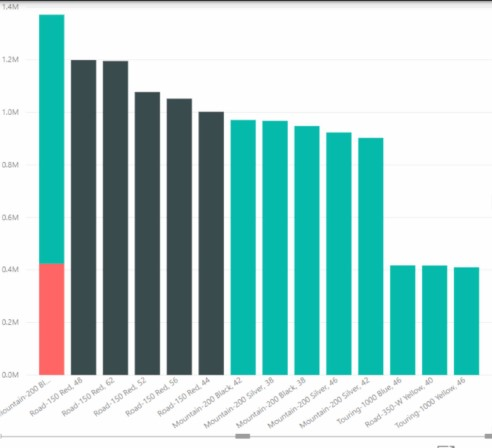
\includegraphics[width=7cm]{./IMAGENES/16} \\
			
			
			Ahora incluya un filtro. Buscaremos productos que hayan vendido arriba de los $400,000
			
			
			
			
			\\ \itemPaso 17: Incluya un Table con los siguientes campos: Sales Amount, English Product Name y Calendar Year Seleccione Show Data
				\\ 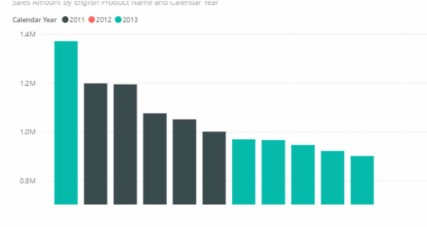
\includegraphics[width=7cm]{./IMAGENES/17} \\
			
			
			Podrâ visualizar el detalle de ventas
			
			
			
			
			\\ \item Paso 18: Cambie la orientacién del reporte:
			
			Show data Copy	$
			
				\\ 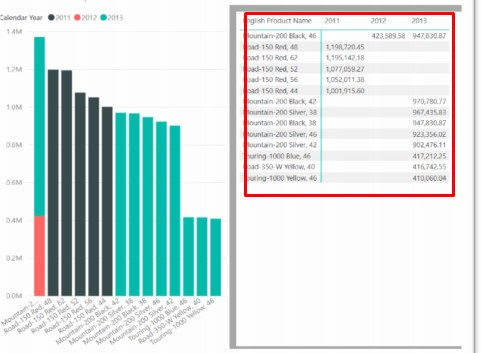
\includegraphics[width=7cm]{./IMAGENES/18} \\
			
			\\ \item Paso 19: Exporte su reporte para visualizacién
			
				\\ \includegraphics[width=7cm]{./IMAGENES/19} \\
			
			
			Utilizando la base de datos Chinook, investigue cémo generar la dimensién de tiempo y luego, crear los siguientes reportes (tome en cuenta que se necesita conocer los valores en dinero):
			
			\\
			Se requiere saber cuâles son los artistas que mas han vendido en la plataforma
			\\ \item 	Ventas por pals contra año
			\\ \item 	Ventas por pals (mapa)
			\\ \item 	Ventas realizadas por artista y año.
			\\ \item 	Genere 4 reportes adicionales utilizando los datos que usted considere relevantes.
			\\ \item 	Investigue cémo visualizar los reportes que ha creado en dispositivos méviles.
			
			
			
		\end{itemize}
	
	
\section
%%INICIO Introducción

\section{Conclusiones}
		\begin{itemize}
		\item Se realizaron con exito  los pasos de la guia, con el fin de concretar conocimiento ya adquiridos en el laboratorio anterior, analizando las ventas y creando tipos de gráficos por cada necesidad de investigador que surga
		\end{itemize}
\section
%%----------------------------------------------------------------------------------------------------------------------------------------------------------



%CONCLUSIONES







	
	
%\citep{referenciarobles2}  


\end{document}

